% Notes:
% 
% The process of decomposing a two-way table (matrix) into two component
% matrices is called singular value decomposition (SVD), which is essentially the reverse process of
% matrix multiplication (from GGE
%
%
%
%
%

\documentclass[serif]{beamer}

% My beamer theme
\usetheme{Hannover}
\usecolortheme{crane}
\definecolor{gray10percent}{RGB}{229, 229, 229}
\definecolor{blockgray}{RGB}{198,188,169}

% My packages
\usepackage{amsmath}
\usepackage{graphicx}
\usepackage{rotating}
\usepackage{etoolbox}

\usepackage{color}
\usepackage{listings}
\lstset
{
	language=C,
	captionpos=b,
	tabsize=3,
	keywordstyle=\color{blue},
	commentstyle=\color[rgb]{0.133,0.545,0.133},
	stringstyle=\color{red},
	breaklines=true,
	showstringspaces=false,
	basicstyle=\footnotesize,
	emph={label},
	keepspaces=true,
	emph={H,G,X,K,KPC},
    emphstyle={\bfseries}
}
\newcommand{\codepause}{\pause \vspace{-0.165in} } 
		


% Decide if you want notes shown
\newtoggle{useNotes}
%\toggletrue{useNotes}
\togglefalse{useNotes}

\iftoggle{useNotes}
{
	\usepackage{pgfpages}
	\setbeameroption{show notes on second screen}
}


% Title Page definition
\title
{
	KPCA-Biplots
}
\subtitle{An implementation and further exploration}
\author
{
	Michael Semeniuk, Albert Steppi, and \linebreak
	Christopher Wolas
}
\date
{
	\begin{block}{}
	\begin{itemize}
		\item
		{
			\underline{Mining Gene Expression Profiles: An Integrated} \linebreak
			\underline{Implementation of Kernel Principal Component} \linebreak
			\underline{Analysis and Singular Value Decomposition}
			\begin{itemize}
					\item  Reverter et al,Genomics Proteomics Bioinformatics (2010)
			\end{itemize}
		}
	\end{itemize}	
	\end{block}
	
}

\begin{document}
	
	\section{Problem Domain}
	
	\begin{frame}
		\titlepage
		
		\note
		{
			TODO
		}		
	\end{frame}

	\begin{frame}[t]
	\frametitle{Simplified Problem Domain Explanation}
		Understanding of our problem domain is as easy as... \linebreak
		\uncover<1-> {1, }
		\uncover<2-> {2, }
		\uncover<3>  {3}
		\begin{columns}[t]
		
			\column{2in}
			{
				\only<1>
				{
					\begin{block}
					{ 
						Analyze Microarray Expression Profiles Relationships
					}
					{
						Extract the highly \underline{non-linear} relationships
						between gene expression profiles and disease 
						classification using \textbf{modern machine learning} techniques.	
					}
					\end{block}
				}
				\only<2>
				{
					\begin{block}
						{ 
							Visualize These Relationships
						}
						{
							Use specialized graphs called \textbf{biplots}
							which plot \emph{both} the gene intensities and classifications on the same $R$-dimensional plane.
						}
					\end{block}
				}
				\only<3>
				{
					\begin{block}
					{
						Interepret relationships and focus on
						a specialized problem						
					}
					{
						\footnotesize 
						Find meaningful results such as:
						\begin{itemize}
							\item Gene Up/Down-\linebreak 
							Regulation in certain diseases
							\item Classifying novel Gene Profiles based on
							analyzed data
						\end{itemize}
						This \emph{can} lead to \underline{seperate} specialized
						research topics.
					}
					\end{block}
				}
			}
			\column{1in}
			{
				\only<1>
				{
					\begin{center}
						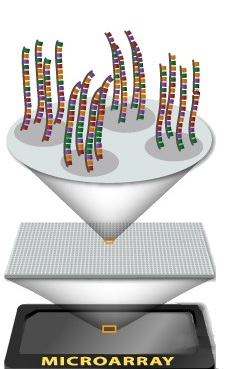
\includegraphics[width=1in]{images/microarray}	
					\end{center}
				}
				\only<2>
				{
					\vspace{0.5in}
					\textbf{IMAGE OF BIPLOT}
				}
				\only<3>
				{
					\vspace{-0.10in}
					\begin{center}
						
\includegraphics[width=1in]{images/meme_face}
					\end{center}
				}
			}
		\end{columns}
		
		\note
		{
			
		}
		
	\end{frame}
	
	\begin{frame}[t]
		\frametitle
		{
			``Microarray analysis? \linebreak
		}
		\framesubtitle
		{		
			\vspace{-0.2in}
			... Isn't that an ancient problem? \linebreak
			Why on earth would you do that...?!''
		
		}
		
		\begin{itemize}
			
			\item
			{
				\color<2-3>{gray10percent}
				{
					By using more sophisticated techniques (non-linear machine
					learning) we can extract \underline{higher fidelity results}
					on the same data which can lead to better insights.
				}
			}
			\item
			{
				\color<1,3>{gray10percent}
				{
					An \underline{approachable problem} that gives an
					introductory taste of bioinformatics for
					machine learning students unfamiliar with it.
				}
			}
			\item
			{
				\color<1-2>{gray10percent}
				{
					Problem in the realm of \underline{exploratory statistics}
					which help us understand the large and intricate data 
					we're working with.
				}
			}
		\end{itemize}
		
		
		\note
		{
			Dr. Hu made a comment on this being an old problem. Disspell
			any further implication that we're just doing a meaningless project
			that has no further value to be extracted from it.
		}
	\end{frame}
	
	\section{Algorithm}
	\subsection{Problem Specification}

	\begin{frame}
		\frametitle{KPCA-Biplot Algorithm}
		\subtitle{Problem Formulation}
		
		Start with a Gene Expression Profile matrix $\mathbf{X}$:

		% This is the crazy gene expression matrix with annotations
		\begin{equation}			
		\begin{matrix}
                            % Column anotation
		& & \mathbin
					{ 
						\color[rgb]{0.133,0.545,0.133}\text{Columns represent}
					} 
					& & \\
		& & \mathbin
					{
						\color[rgb]{0.133,0.545,0.133}\text{gene expression intensities}
					}
					& & \\
		& & \rotatebox[origin=c]{270}
			{
				$\begin{cases} 
				& \\ & \\ & \\ & \\ &  \\ & \\ &  \\  & \\ 
				\end{cases}$
			} 
		& & \\
		% Gene expression Matrix 'X'
		&\mathbf{X}=  
		&	\begin{bmatrix}
				x_{1,1} & x_{1,2} & x_{1,3} & \ldots  & x_{1,p} \\ 
				x_{2,1} & x_{2,2} & x_{2,3} & \ldots  & x_{2,p} \\ 
				x_{3,1} & x_{3,2} & x_{3,3} & \ldots  & x_{3,p} \\ 
				\vdots  & \vdots  & \vdots  & \ddots  &         \\ 
				x_{n,1} & x_{n,2} & x_{n,3} &         & x_{n,p} \\ 
			\end{bmatrix}
                            % Row Anotation
		&\left.
			\begin{matrix}
				\\ \\ \\ \\ \\  
			\end{matrix}
		 \right\}
        & \rotatebox[origin=c]{0}
        	 {
        	 	$\begin{matrix} 
                    \mathbin
                    {
                    	\color[rgb]{0.133,0.545,0.133}\text{Rows}
					  }\\
	          		  \mathbin
	          		  {
	          		  	\color[rgb]{0.133,0.545,0.133}\text{represent}
	          		  }\\
	          		  \mathbin
	          		  {
	          		  	\color[rgb]{0.133,0.545,0.133}\text{labeled}
	          		  } \\ 
	          		  \mathbin
	          		  {
	          		  	\color[rgb]{0.133,0.545,0.133}\text{samples}
	          		  } \\ 
          		  \end{matrix}$
      		  } \\

		\end{matrix}
		\end{equation}
		
	\end{frame}
	
	\begin{frame}
		\frametitle{}
			\begin{block}{Terminology Notes:}
			\begin{itemize}
				\item 
				{
					\color<2,3>{blockgray}
					{
						Gene expression intensities are measurements
						of the activity of each gene.\newline
					}
				}
				\item 
				{
					\color<1>{blockgray}
					{
						They can tell us:
					}
					
					% WOW, this is super wordy. I want to say this more succinctly.
					% Explain what a condition could be: Abnormality, Disease, Syndrome, identifiable trait(?)
					\begin{enumerate}
						\item
						{
							\color<1,3>{blockgray}
							{
								Upregulation or downregulation of genes
								depending if certain condition is expressed.
							}
						}
						\item
						{				
							\color<1,2>{blockgray}
							{
								Collectively, they can form gene expression
								profiles which can identify an indivdual 
								with a condition.
						    }
						}
					\end{enumerate}
				}
			\end{itemize}
				
				
			\end{block}
			
	\end{frame}
	
	\subsection{Preprocessing}
	
	\begin{frame}[fragile,t]
		\frametitle{KPCA-Biplot Algorithm}
		\framesubtitle{Preprocessing}
		Next, perform preprocessing. \newline

		\begin{lstlisting}[mathescape]
		for(i $\ldots$ N)
		{
		    // Where $T_{i}$(...) is some preprocessing function
		    // which transforms a vector into a new one.	
		    $\mathbf{X}=T_{i}(\mathbf{X})$
		}
		\end{lstlisting}	
		
		\note
		{

		}
	\end{frame}

	\begin{frame}
		\begin{block}{Notes:}
			
			Several established techniques are as follows:
			
			\begin{enumerate}
				\item
				{
					\color<2->{blockgray}
					{
						Normalization (e.g. $\log$ transformation)
					}
				}
				\item
				{	
					\color<1,3->{blockgray}
					{					
						Gene Centering (subtract $\mu$
						intensity of gene from each gene)
					}
				}
				\item
				{
					\color<1-2,4->{blockgray}
					{
						Gene Scaling (by standard deviation)
					}
				}
				\item
				{
					\color<1-3,5>{blockgray}
					{
						Filters
					}
					\begin{enumerate}
						\item
						{
							\color<1-3,5>{blockgray}
							{
								Simple threshold filters
							}
						}
						\item 
						{
							\color<1-3,5>{blockgray}
							{
								Interquartile Range filters
							}
						}
						\item
						{
							\color<1-3,5>{blockgray}
							{
								ANOVA fitlers
							}
						}
					\end{enumerate}
				}
				\item 
				{
					\color<1-4>{blockgray}
					{
						Sample Removal
					}
					\begin{enumerate}
						\item
						{
							\color<1-4>{blockgray}
							{
								Errorneous samples
							}
						}
						\item
						{
							\color<1-4>{blockgray}
							{
								Incomplete samples
							}
						}
						\item
						{
							\color<1-4>{blockgray}
							{
								Sample of a classification with not enough samples
							}
						}
					\end{enumerate}
				}
			\end{enumerate}
		\end{block}
		
	\end{frame}

	\subsection{SVD}

	\begin{frame}[fragile,t]
		\frametitle{KPCA-Biplot Algorithm}
		\framesubtitle{Singular Value Decomposition \textbf{(SVD)}}
		Now perform singular value decomposition. \newline
		
		
		\begin{lstlisting}[mathescape, language=C]
		// Decompose matrix X into 3 parts using SVD:
		// U = Unitary matrix
		\end{lstlisting}
		\codepause
		\begin{lstlisting}[mathescape, language=C]
		// D = rectangular diagonal matrix (with
		//       positive real numbers)
		\end{lstlisting}
		\codepause 
		\begin{lstlisting}[mathescape, language=C]
		// $\mathbin{ \color[rgb]{0.133,0.545,0.133} V^{T}}$ = conjugate transpose of V (a unitary matrix)
		\end{lstlisting}
		\codepause
		\begin{lstlisting}[mathescape, language=C]
		$ U D V^{T} =$ X
		\end{lstlisting}
		\codepause
		\begin{lstlisting}[mathescape, language=C]
		
		// Get the expression in terms of G and H:
		GH$^{T}$ = $U D^{\alpha} D^{(1 - \alpha)} V^{T}$ = $U D V^{T}$ = X 
		\end{lstlisting}
		\codepause
		\begin{lstlisting}[mathescape, language=C]
		
		// Decompos. of Rows Effects (Microarray Samples):
		G = $U \times D^{\alpha}$ 	
		\end{lstlisting}
		\codepause
		\begin{lstlisting}[mathescape, language=C]
		
		// Decompos. of Column Effects (Gene Expressions):
		H$^{T}$ = $V^{T} \times D^{(1-\alpha)}$	
		\end{lstlisting}
	\end{frame}

	\begin{frame}
		\begin{block}{TODO SVD:}
			\begin{itemize}
				\item  Explain SVD (high level with perhaps some math and handwaving)
				\item  visualization of SVD (in terms of affine transforms)
				\item  I like http://nimbledais.com/?p=57
			\end{itemize}
		\end{block}
		\begin{center}
			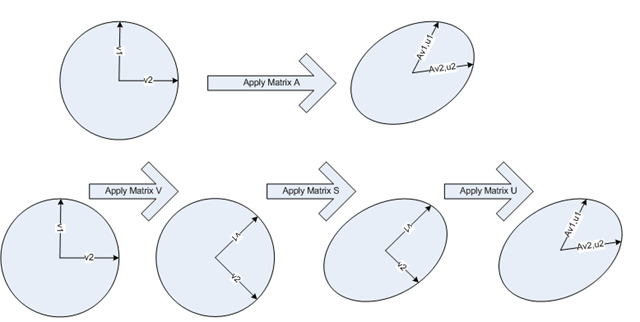
\includegraphics[width=2in]{images/svd_intuitive}	
		\end{center}
		
	\end{frame}
	
	\begin{frame}
		\begin{block}{TODO $\alpha$:}
			Explain $\alpha$ and its purpose
		\end{block}
	\end{frame}
	
	\subsection{Kernel Matrix}
	
	\begin{frame}[t, fragile]
		\frametitle{KPCA-Biplot Algorithm}
		\framesubtitle{Finding the Kernel Matrix}
		
		Compute the Kernel Matrix.
		
		\begin{lstlisting}[mathescape, language=C]
		
		// Use the radial basis kernel which takes the form:
		//  $\mathbin{ \color[rgb]{0.133,0.545,0.133} K(x,y) = exp(-\frac{{ \left\| x-y \right\|  }^{ 2 }}{2\sigma^{2}})}$
		// 
		// 
		//
		//
		//
		//
		\end{lstlisting}
		% Let's be clever and make an image comment lol
		\vspace{-1.10in}
		\begin{center}
		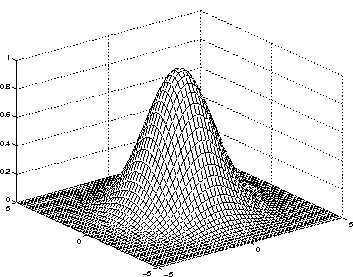
\includegraphics[width=1.0in]{images/rbf_kernel}	
		\end{center}
		\vspace{-0.07in}
		\codepause
		\begin{lstlisting}[mathescape, language=C]
		// We will be computing the kernel matrix using our
		// radial basis kernel for H (the gene expressions)
		K = Find_Kernel_Matrix(kernel_function=$K_{\text{radial basis}}(x,y)$,
		                       dataset=H,
		                       $\sigma$ = To be determined )
		
		\end{lstlisting}

	\end{frame}
	
	\begin{frame}
		\begin{block}{Notes on Kernel:}
			% Quoting paper
			\begin{itemize}
			\item
			{
			\color<2-4>{blockgray}
			{
				Kernel function choice is critical since the kernel
				uses it as a similarity metric.
			}
				\begin{itemize}
					\item
					{
						\color<1,3-4>{blockgray}
						{
							Two natural candidates were considered:
						}
							\begin{enumerate}
							
								\item
								{ 
									\color<1,3-4>{blockgray}{Polynomial Kernel}
								}
								\item
								{ 
									\color<1,3-4>{blockgray}{Radial Basis Kernel}
								}
							\end{enumerate}
						
					}
					\item
					{
						\color<1-2,4>{blockgray}
						{
							\textbf{Radial Basis Kernel} was found 
							to do \underline{better} and is used.
						}
					}
				\end{itemize}
			}
			\item
			{
				\color<1-3>{blockgray}
				{
					Kernel tuning parameters are also \underline{critical} 
					(e.g. $\sigma$ value). This will be further 
					explored \emph{later}.
				}
			}
			\end{itemize}
		\end{block}
	\end{frame}
	
	\subsection{KPCA}
	
	\begin{frame}[t, fragile]
		\frametitle{KPCA-Biplot Algorithm}
		\framesubtitle{Kernel Principal Component Analysis \textbf{(KPCA)}}
		
		Perform Kernel Principal Component Analysis.
		
	\begin{lstlisting}[mathescape, language=C]
		// Extract the nonlinear features of gene expression 
		// matrix H by computing the first 2 principal 
		// components using the Kernel Matrix
		KPC$_{H}$ = Do_KPCA(num_of_principal_components = 2,
		               kernel_matrix = K)
	\end{lstlisting}

	\end{frame}

	\begin{frame}
		\begin{block}{KPCA TODO:}
			\begin{itemize}
			\item  Some explanation of PCA (intuitive but mathematical, perhaps)
			\item  Extension from PCA to KPCA
			\item  Explanation of why \emph{2} Kernel Principal Components (visualizable graphical output)	
			\end{itemize}
		\end{block}
	\end{frame}

	\subsection{Projection}
	
	\begin{frame}[t, fragile]
		\frametitle{KPCA-Biplot Algorithm}
		\framesubtitle{Subspace Projection}
		
		\begin{lstlisting}[mathescape, language=C]
		// Compute a second Kernel Matrix for both the Gene
		...
		\end{lstlisting}
		\codepause
		\begin{lstlisting}[mathescape, language=C]
		
		// Project the microarrays G onto the subspace
		G$_{Projection}$ = K$^{T} \times $ KPC$_{ H }$
		\end{lstlisting}		
	\end{frame}
	
	\begin{frame}
		\begin{block}{Subspace Projection TODO:}
			\begin{itemize}
				\item  Write how it works
			\end{itemize}
		\end{block}
	\end{frame}
	
	\subsection{Biplot}

	\begin{frame}[t, fragile]
		\frametitle{KPCA-Biplot Algorithm}
		\framesubtitle{Biplot}
		
		\begin{lstlisting}[mathescape, language=C]
		
		// Classification of each microarray sample row
		File$_{Classification}$ = Read_Classifications(...)
		\end{lstlisting}
		\codepause
		\begin{lstlisting}[mathescape, language=C]
		
		// Metadata about each gene column
		File$_{Genes}$= Read_Gene_Metadata(...)
		\end{lstlisting}
		\codepause
		\begin{lstlisting}[mathescape, language=C]
		
		// Plot your biplot with the collected data
		GE_Biplot(gene_expressions = G$_{Proj}$,
		          gene_metadata = File$_{Genes}$=,
		          microarray_samples = H,
		          microarray_classification = File$_{Classification}$)
		\end{lstlisting}
		\begin{lstlisting}[mathescape, language=C]
		>>
		>>
		>>
		>> 
		>>
		>>
		\end{lstlisting}
		% Let's be clever and make an image comment lol
		\vspace{-1.17in}
		\begin{center}
		\raggedright \hspace{0.2in}
		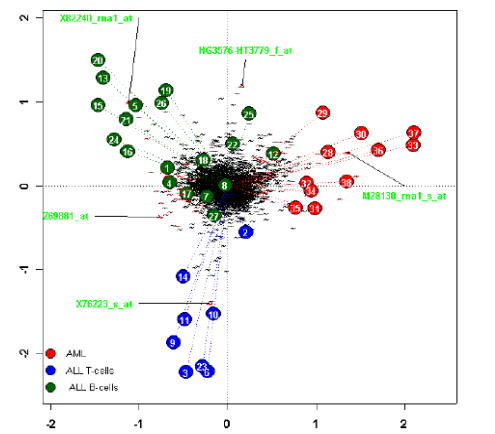
\includegraphics[width=1.0in]{images/biplot_output}	
		\end{center}
		\codepause
		
		
	\end{frame}
	
	\section{Datasets}
	\begin{frame}
		\frametitle{KPCA-Biplot}

		In our research we've used {\bf 4} freely available datasets with labeled samples:

		% http://icos.cs.nott.ac.uk/datasets/microarray.html
		% http://www.inf.ed.ac.uk/teaching/courses/dme/html/datasets0405.html
		\begin{enumerate}
			\item {\bf COLON dataset}: 
				\begin{itemize}
					\item  $ Labels = \left \{ \text{Tumor}, \text{No Tumor}  \right \}$
					\item 2,000 gene expression levels, 62 samples
				\end{itemize}
			\item {\bf LYMPHOMA dataset}: 
				\begin{itemize}
					\item  $ Labels = 
						\left \{ \text{DLBCL}\footnote{Diffuse large B-cell lymphoma},
							 \text{FL}\footnote{Follicular lymphoma}  \right \}$
					\item 6,817 gene expression levels, 77 samples % DLBCL (n = 58) and FL (n = 19)
				\end{itemize}
			\item {\bf PROSTATE dataset}:
				\begin{itemize}
					\item  $ Labels = \left \{ \text{Tumor}, \text{No Tumor}  \right \}$
					\item 2,135 gene expression levels, 77 samples % Tumor (n = 52) and No Tumor (n = 50)
				\end{itemize}
			% http://www.biolab.si/supp/bi-cancer/projections/info/leukemia.htm
			\item {\bf Leukemia dataset }:
					\begin{itemize}
					\item  $ Labels = 	\left
						 \{ \text{ALL}\footnote{Acute lymphoblastic leukemia},
						 \text{AML}\footnote{Acute myeloid leukemia}
								 \right \}$
					\item 5,147 gene expression levels, 72 samples % ALL (n = 47) and AML (n = 25)
				\end{itemize}
		\end{enumerate}		

	\end{frame}

	\begin{frame}
		How they were preprocessed
	\end{frame}

	\subsection{Tuning}
	\begin{frame}
		Wait a minute, what about the unsolved parameters?
	\end{frame}
	
	\begin{frame}
		\begin{block}{Optimization Parameters:}
			\begin{itemize}
				\item  $\alpha$ - ...
				\item  $\sigma$ - ...
			\end{itemize}
		\end{block}	
	\end{frame}
	
	\begin{frame}
		Example of different alpha values ( 0.00, 0.10, 0.20, 0.30, 0.40)
	\end{frame}
	
	\begin{frame}
		Example of different alpha values ( 0.50, 0.60, 0.70, 0.80, 0.90, 1.00)
	\end{frame}
	
	\subsection{Validation}
	\begin{frame}
		Discussion of kernel tuning and cross validation 
	\end{frame}
	
	\begin{frame}
		Insert pseudocode for cross validation algorithm
	\end{frame}
	
	\begin{frame}
		Insert our optimized sigma values versus theirs
	\end{frame}
	
	
	\section{Results}
	
	\begin{frame}
		COLON Results (Our KPCA-Biplot vs Reverter KPCA)
	\end{frame}
	
	\begin{frame}
		COLON Results (Our KPCA-Biplot vs Biplot)
	\end{frame}
	
	\begin{frame}
		LYMPHOMA Results (Our KPCA-Biplot vs Biplot)
	\end{frame}
	
	\begin{frame}
		PROSTATE Results (Our KPCA-Biplot vs Biplot)
	\end{frame}
	
	\begin{frame}
		LEUKEMIA RESULTS (Our KPCA-Biplot vs Reverter KPCA)
	\end{frame}	
	
	\begin{frame}
		LEUKEMIA RESULTS (Our KPCA-Biplot vs Biplot)
	\end{frame}

	\begin{frame}
		How to interpret biplots (take from albert's slides)
	\end{frame}
	
	
	\section{Analysis}
	
	\begin{frame}
		Individual analysis of genes. We can say we still haven't finished but
		we'll put it in the report.
	\end{frame}
	
	\begin{frame}
		Insert what genes Reverter et Al. found expressed
	\end{frame}
	
	
	\section{Program}
	
	\begin{frame}
		Implementation in R, Python (import picture logos, very brief talking points). Necessary because we did do an implementation so code DOES
		matter.
	\end{frame}
	
	
	\section{Insights}
	
	\begin{frame}
		Insights:
		\begin{itemize}
			\item  Datasets were computationally expensive
			\item  Literature on biplots was esoteric
			\item  No cross validation methodology revelead (had to
			replicate using techniques determined within team)
			\item  No KPCA-Biplot code freely available (had to implement
			using paper)
			\item  Exploratory statistics is a new topic to us
		\end{itemize}
	\end{frame}
	
	\section{Extensions}
	
	\begin{frame}
		Authors had no extensions listed. Here's some:
		\begin{itemize}
			\item  Algorithm to select highly differentiable genes automatically
			using the intrinsic relationships of biplots
			\item  Algorithm to find the best alpha for biplot
			\item  Goodness of Fit metrics for biplots
		\end{itemize}
	\end{frame}
	
	\begin{frame}
		Fin
	\end{frame}

	\begin{frame}
		Bib
	\end{frame}
	
\end{document}